\section{Mobile Application}
\label{sec:mobile_application}

The mobile application serves as the central user interface of our AI-powered respiratory analysis system. Built with Flutter, it offers a seamless and cross-platform experience. This section presents a walkthrough of the app’s core features, showcasing its design, functionality, and user flow.

\subsection{Visual Identity and Design Language}

The application embraces a medically inspired color palette referencing the official World Health Organization (WHO) guidelines, aiming for clarity, trust, and accessibility. The logo symbolizes the lungs through a stylized graphic, while the central dot represents a sensor tasked with detecting respiratory anomalies.

The primary branding elements, including both filled and outline logo variants, are shown in Figure~\ref{fig:app_logos}.

\begin{figure}[H]
    \centering
    
\includegraphics[width=0.25\textwidth]{images/UI_Screenshots/logo_filled.png}
    \hspace{2em}
    
\includegraphics[width=0.25\textwidth]{images/UI_Screenshots/logo_unfilled.png}
    \caption{Application Logos: Filled and Outline}
    \label{fig:app_logos}
\end{figure}

\subsection{Authentication: Login and Signup}

The user journey begins with secure authentication. A simple interface for logging in or signing up is provided, as seen in Figure~\ref{fig:login_screen}.

\begin{figure}[H]
    \centering
    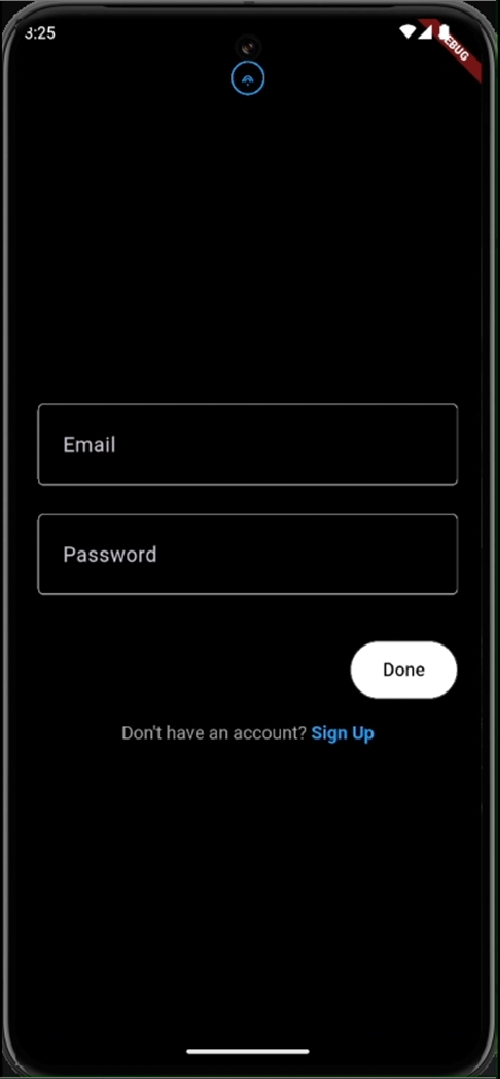
\includegraphics[width=0.35\textwidth]{images/UI_Screenshots/login_screen.png}
    \caption{Login Screen}
    \label{fig:login_screen}
\end{figure}

\subsection{User Profile Management}

Once authenticated, users are directed to a profile screen where they can view and manage their personal information. This interface is illustrated in Figure~\ref{fig:profile_screen}.

\begin{figure}[H]
    \centering
    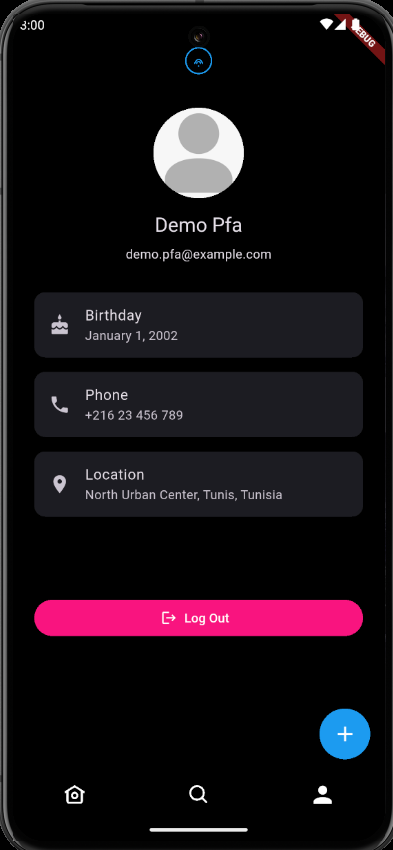
\includegraphics[width=0.35\textwidth]{images/UI_Screenshots/profile_screen.png}
    \caption{Profile Screen}
    \label{fig:profile_screen}
\end{figure}

\subsection{Home Screen – No Diagnoses Yet}

The initial home screen is presented when the user has not yet submitted any diagnoses. This clean interface is displayed in Figure~\ref{fig:home_screen_empty}.

\begin{figure}[H]
    \centering
    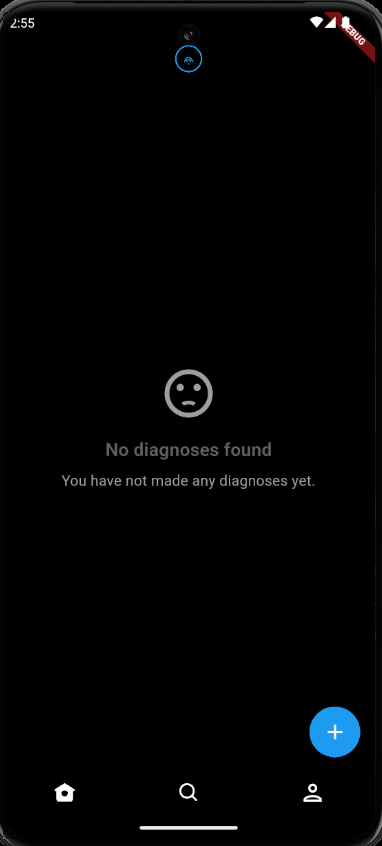
\includegraphics[width=0.35\textwidth]{images/UI_Screenshots/home_screen_no_diagnoses.png}
    \caption{Home Screen Without Diagnoses}
    \label{fig:home_screen_empty}
\end{figure}

\subsection{Search Screen – No History}

A search feature is available for reviewing past diagnoses. In the absence of history, the interface appears as shown in Figure~\ref{fig:search_screen_empty}.

\begin{figure}[H]
    \centering
    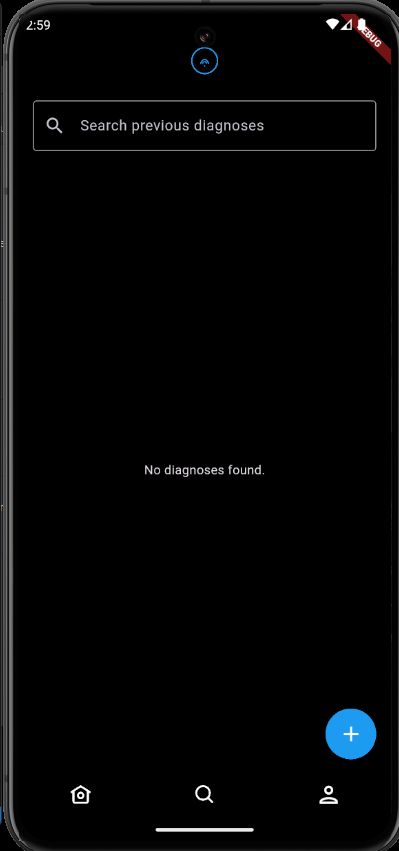
\includegraphics[width=0.35\textwidth]{images/UI_Screenshots/search_screen.png}
    \caption{Search Screen Without History}
    \label{fig:search_screen_empty}
\end{figure}

\subsection{Creating a New Diagnosis}

To start a diagnosis, users can record audio, upload medical files, and input symptoms using the interface shown in Figure~\ref{fig:create_diagnosis}.

\begin{figure}[H]
    \centering
    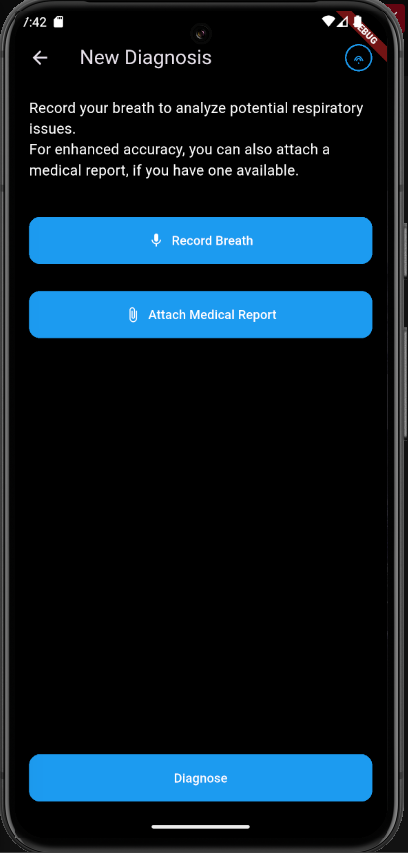
\includegraphics[width=0.35\textwidth]{images/UI_Screenshots/create_diagnosis_screen.png}
    \caption{Diagnosis Creation Interface}
    \label{fig:create_diagnosis}
\end{figure}

\subsection{Home Screen – With Previous Diagnoses}

After a diagnosis is performed, the home screen updates to reflect the user's diagnostic history, as demonstrated in Figure~\ref{fig:home_screen_with_history}.

\begin{figure}[H]
    \centering
    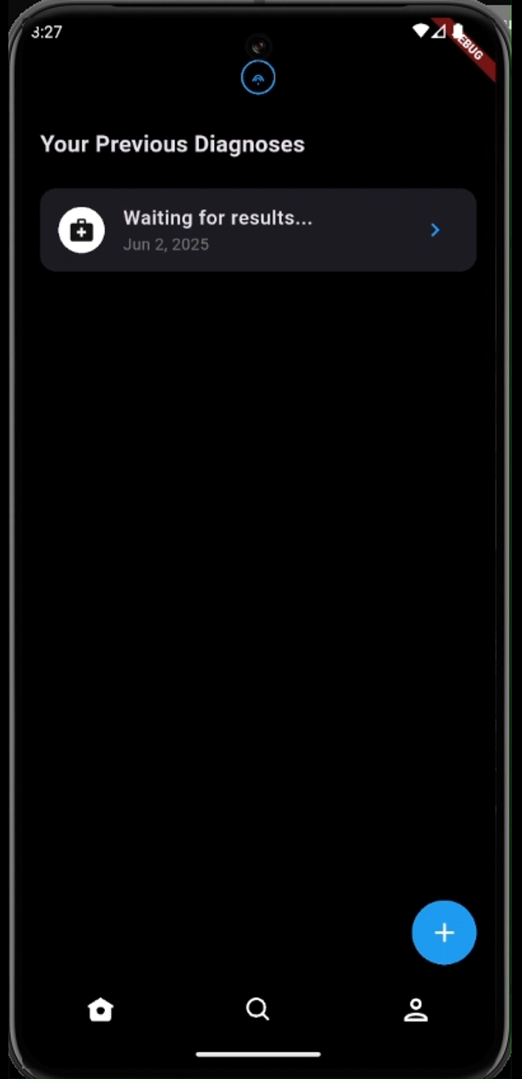
\includegraphics[width=0.35\textwidth]{images/UI_Screenshots/home_screen_with_previous_diagnoses.png}
    \caption{Home Screen Displaying Previous Diagnoses}
    \label{fig:home_screen_with_history}
\end{figure}

\subsection{Diagnosis Details – Waiting for Results}

Once a new diagnosis is submitted, the system informs the user that the analysis is in progress. This intermediate state is depicted in Figure~\ref{fig:diagnosis_waiting}.

\begin{figure}[H]
    \centering
    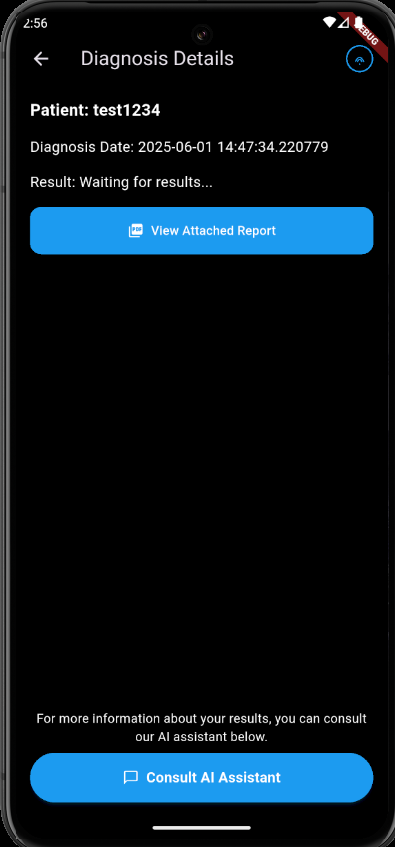
\includegraphics[width=0.35\textwidth]{images/UI_Screenshots/diagnosis_details_screen_waiting_for_results.png}
    \caption{Diagnosis Details – Awaiting AI Analysis}
    \label{fig:diagnosis_waiting}
\end{figure}

\subsection{Diagnosis Details – Results Ready}

After analysis is complete, users are presented with detailed diagnostic feedback, as shown in Figure~\ref{fig:diagnosis_results}.

\begin{figure}[H]
    \centering
    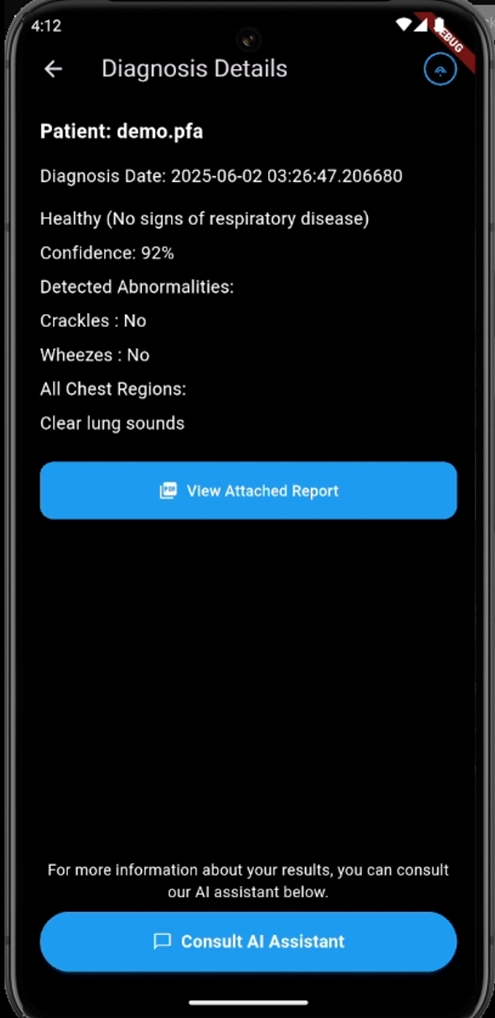
\includegraphics[width=0.35\textwidth]{images/UI_Screenshots/diagnosis_details_screen_results_ready.png}
    \caption{Diagnosis Details – Results Ready}
    \label{fig:diagnosis_results}
\end{figure}

\subsection{AI Assistant Onboarding}

When consulting the AI assistant for the first time, users are guided through an onboarding screen that outlines its purpose, as illustrated in Figure~\ref{fig:ai_onboarding}.

\begin{figure}[H]
    \centering
    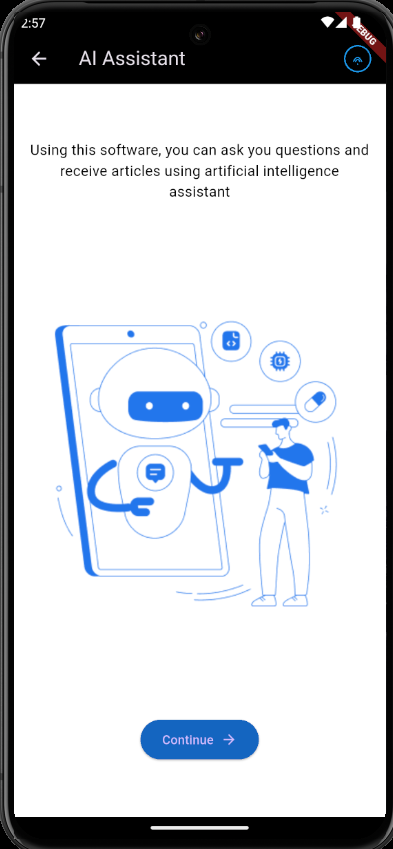
\includegraphics[width=0.35\textwidth]{images/UI_Screenshots/on_boarding_ai_assistant_screen.png}
    \caption{AI Assistant Onboarding Screen}
    \label{fig:ai_onboarding}
\end{figure}

\subsection{AI Assistant – Start Screen}

Following onboarding, users arrive at a starting interface that invites medical queries, as depicted in Figure~\ref{fig:ai_start}.

\begin{figure}[H]
    \centering
    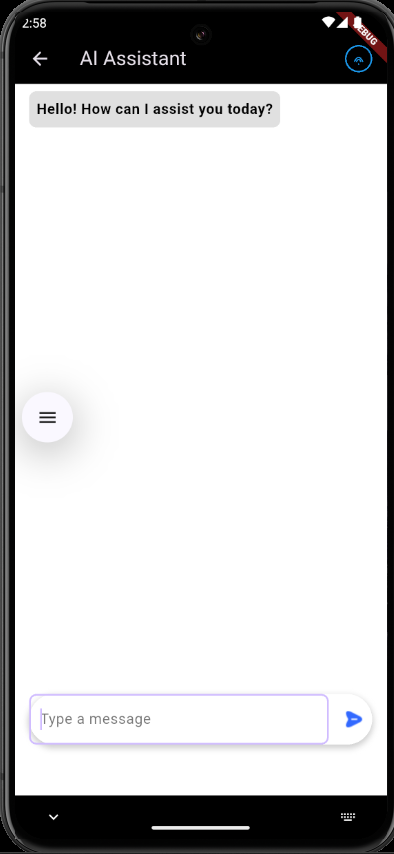
\includegraphics[width=0.35\textwidth]{images/UI_Screenshots/ai_assistant_screen_starting_screen.png}
    \caption{AI Assistant – Starting Interface}
    \label{fig:ai_start}
\end{figure}

\subsection{AI Assistant – Chat Interface}

The assistant responds in a conversational style, as shown in Figure~\ref{fig:ai_chat}, providing interactive, medically grounded guidance.

\begin{figure}[H]
    \centering
    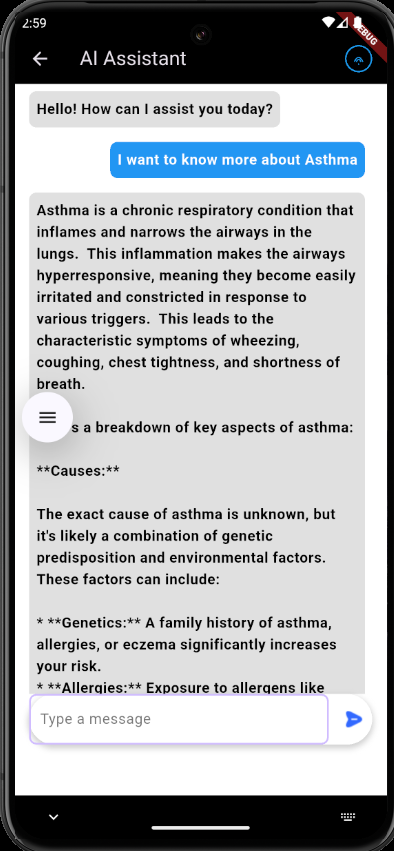
\includegraphics[width=0.35\textwidth]{images/UI_Screenshots/ai_assistant_screen_chat_example.png}
    \caption{AI Assistant Chat Interaction}
    \label{fig:ai_chat}
\end{figure}

\subsection{Summary}

The mobile application was designed to deliver a smooth, medically reliable, and user-centric experience. Each screen plays a specific role in guiding the user through authentication, diagnosis creation, result review, and AI consultation. Leveraging Flutter, the app ensures cross-platform consistency and accessibility. The clear design, inspired by WHO standards, and the integration of visual cues like the lung-symbol logo reinforce its identity as a trusted respiratory health tool.
